\documentclass[12pt,a4paper]{article}

\usepackage[margin=1in]{geometry}
\usepackage[T1]{fontenc}
\usepackage[utf8]{inputenc}
\usepackage{lmodern}
\usepackage{microtype}
\usepackage{setspace}
\usepackage{graphicx}
\usepackage[table]{xcolor}
\usepackage{booktabs}
\usepackage{array}
\usepackage{longtable}
\usepackage{tabularx}
\usepackage{enumitem}
\usepackage{caption}
\usepackage{subcaption}
\usepackage{float}
\usepackage{hyperref}
\usepackage{tikz}
\usepackage{pgfplots}
\usepackage{titlesec}

\pgfplotsset{compat=1.18}
\usetikzlibrary{arrows.meta,positioning,shapes.geometric,fit}

\definecolor{safargreen}{HTML}{1A6B3C}
\definecolor{headingblue}{HTML}{0F2E5F}
\definecolor{subheadingblue}{HTML}{1D4ED8}
\definecolor{safaryellow}{HTML}{F59E0B}
\definecolor{safarred}{HTML}{DC2626}
\definecolor{safargray}{HTML}{6B7280}
\definecolor{safarblue}{HTML}{2563EB}
\definecolor{lightgreen}{HTML}{ECFDF3}
\definecolor{lightyellow}{HTML}{FFFBEB}
\definecolor{lightred}{HTML}{FEF2F2}
\definecolor{lightgray}{HTML}{F3F4F6}

\hypersetup{
  colorlinks=true,
  linkcolor=headingblue,
  citecolor=headingblue,
  urlcolor=safarblue,
  pdftitle={SafarSathi: Mountain Travel Safety System for Mandi Region},
  pdfauthor={Arman Rawat, Gaurav Ahuja, Tanish Kumar, Anuj Aggarwal}
}

\setstretch{1.12}
\setlist[itemize]{leftmargin=1.4em,itemsep=0.25em,topsep=0.3em}
\setlist[enumerate]{leftmargin=1.6em,itemsep=0.25em,topsep=0.3em}
\titleformat{\section}{\large\bfseries\color{headingblue}}{\thesection}{0.75em}{}
\titleformat{\subsection}{\normalsize\bfseries\color{subheadingblue}}{\thesubsection}{0.75em}{}
\titleformat{\subsubsection}{\normalsize\bfseries\itshape\color{subheadingblue}}{\thesubsubsection}{0.75em}{}

\newcommand{\risklow}{\cellcolor{lightgreen}\textbf{LOW}}
\newcommand{\riskmed}{\cellcolor{lightyellow}\textbf{MEDIUM}}
\newcommand{\riskhigh}{\cellcolor{lightred}\textbf{HIGH}}
\newcommand{\riskunknown}{\cellcolor{lightgray}\textbf{UNKNOWN}}

\newcommand{\maybeimage}[4]{%
  \IfFileExists{#1}{%
    \includegraphics[width=#2,height=#3,keepaspectratio]{#1}%
  }{%
    \fbox{\parbox[c][#3][c]{#2}{\centering\small #4\\[0.35em]\footnotesize\texttt{#1}}}%
  }%
}

\begin{document}

\begin{titlepage}
  \centering
  \vspace*{0.5cm}
  {\Large Indian Institute of Technology Mandi\par}
  \vspace{0.25cm}
  {\large DP301P --- Interactive Socio-Technical Practicum (ISTP)\par}
  {\large Academic Year 2025--2026\par}
  \vspace{1.5cm}
  {\Huge\bfseries SafarSathi\par}
  \vspace{0.35cm}
  {\Large Mountain Travel Safety System for the Mandi Region\par}
  \vspace{0.35cm}
  {\large A multi-channel, offline-first safety information bridge for first-time visitors, parents, and local stakeholders\par}
  \vspace{1.2cm}
  {\large Group No.\ G11\par}
  \vspace{0.9cm}
  \begin{tabular}{>{\bfseries}p{0.34\linewidth}p{0.46\linewidth}}
    Team Members & Arman Rawat \hfill (B22152)\\
                 & Gaurav Ahuja \hfill (B22300)\\
                 & Tanish Kumar \hfill (B22243)\\
                 & Anuj Aggarwal \hfill (B22088)\\[0.5cm]
    Faculty Advisor / Mentor & Dr.\ Mohammad Talha, IIT Mandi\\
    Course & Interactive Socio-Technical Practicum 2026\\
  \end{tabular}
  \vfill
  {\large Submitted on: 26 April 2026\par}
\end{titlepage}

\pagenumbering{roman}
\tableofcontents
\newpage
\listoffigures
\listoftables
\newpage
\pagenumbering{arabic}

% -----------------------------------------------------------------------
\section*{Extended Abstract}
\addcontentsline{toc}{section}{Extended Abstract}

Mountain travel around Mandi, Himachal Pradesh is not unsafe because information is absent. It is unsafe because useful information reaches tourists too late, in the wrong format, or not at all. A taxi driver at Mandi ISBT may know that the road beyond Baggi has washed out, HP SDMA may have published alerts, and IMD may have issued district warnings, but a parent arriving from Delhi or Lucknow often does not know where to look, whom to call, or what to save before entering a low-connectivity road section.

SafarSathi addresses this delivery gap. We built a mountain travel safety system covering three high-use routes from Mandi: Parashar Lake, Barot Valley, and Kullu/Manali via NH-3. The core idea is intentionally simple: combine seasonal route risk, official weather and disaster information, trusted local reports, emergency contacts, and offline preparation guidance, then deliver it through channels tourists already use.

We conducted structured fieldwork with tourists, parents, taxi drivers, dhaba owners, and homestay operators. These conversations directly shaped the design: avoid heavy app installs, prioritise WhatsApp and a QR-opened progressive web app (PWA), and ensure emergency information survives without an internet connection. The resulting system includes a FastAPI backend, a conservative risk engine, IMD/HP SDMA/HP PWD scrapers, a WhatsApp Business bot with keyword-driven route safety responses, a Telegram bot with live polling, SMS fallback logic, and a React PWA with offline route cards, checklists, emergency contacts, altitude sickness guidance, and a MapLibre-based map.

Our risk engine is the main technical contribution. Rather than pretending to provide turn-by-turn navigation or live traffic, it produces a conservative risk level from seasonal baselines, weather freshness, official alerts, verified local reports, time of day, and route-specific terrain. A critical design rule prevents false reassurance: stale data is never treated as ``LOW'' risk. If no fresh report or alert exists outside the best travel window, the system returns ``UNKNOWN'' rather than green.

We deployed the full stack, evaluated it with real users during fieldwork, and built a verified reporter network. SafarSathi demonstrates that a lightweight, locally grounded system can package scattered safety knowledge into a usable decision aid that works even when the internet does not.

% -----------------------------------------------------------------------
\section{Introduction}

\subsection{Background and Context}

Himachal Pradesh depends heavily on road-based mobility. Visitors travel by bus, taxi, private car, and shared vehicles through roads that pass steep slopes, narrow valleys, river gorges, and areas with weak or intermittent mobile connectivity. In the Mandi region, a visitor can move from the relatively accessible town environment to roads where the nearest hospital, petrol pump, phone signal, or police post may be far behind. This is especially visible on routes to Parashar Lake, Barot Valley, and Kullu/Manali.

The risk is seasonal. March to May is usually the clearest travel window. June to September brings monsoon rain, landslides, river swelling, road washouts, and sudden closures. October to February adds cold, short daylight hours, snow or black ice at higher elevations, and visibility problems. HP SDMA's hazard profile identifies landslides, flash floods, snowstorms, avalanches, road accidents, and other hazards as part of the state's risk environment, while Mandi district is among those with very high seismic exposure \cite{hpsdma_hazard}. During monsoon, official updates from HP SDMA have repeatedly documented landslide incidents and blocked roads in and around Mandi, including NH stretches around Pandoh and Aut \cite{hpsdma_incident}. These are not abstract risks; they directly affect visitors who start a trip without checking current conditions.

\subsection{Problem Statement}

Our project began from one practical observation: tourists and parents rarely fail because they do not care about safety. They fail because the safety information pipeline is broken.

Three failures typically appear together:

\begin{itemize}
  \item \textbf{Information asymmetry.} Local drivers and shopkeepers know which stretches are bad, but first-time visitors do not.
  \item \textbf{Accessibility gap.} Official alerts exist, but government websites are not the natural first stop for many tourists, especially older visitors.
  \item \textbf{Connectivity trap.} The road segments where information matters most are often the same places where the internet becomes unreliable.
\end{itemize}

Our key design insight is that this is not mainly a real-time traffic problem. It is an information packaging and delivery problem. The effective intervention is to reach people before they board a bus, before they leave Mandi town, and before the last reliable network point.

\subsection{Research Gap}

Existing travel-safety information is fragmented across weather bulletins, disaster alerts, local knowledge, police contacts, hospital numbers, and informal WhatsApp groups. Navigation tools can show a route, but they do not explain whether a first-time mountain traveller should postpone a monsoon day trip, call a local contact, carry altitude medication, or avoid night travel. Official data sources are trustworthy but not always readable or timely for ordinary visitors. Informal local information is timely but not always structured or accountable.

SafarSathi bridges this gap by building a system that is:

\begin{itemize}
  \item conservative in risk scoring so that doubt is always flagged rather than hidden;
  \item accessible through WhatsApp, Telegram, SMS, PWA, and printed safety cards;
  \item offline-first for emergency contacts, checklists, altitude warnings, and last-connectivity information;
  \item grounded in official sources and a consent-based verified local reporter network;
  \item careful about privacy and data minimisation under India's Digital Personal Data Protection Act, 2023 \cite{dpdp}.
\end{itemize}

\subsection{Objectives}

Our objectives for this project were to:

\begin{enumerate}
  \item identify what first-time visitors and parents actually do before mountain travel around Mandi;
  \item document how local stakeholders currently know and share road conditions;
  \item define seasonal safety baselines for Parashar, Barot, and Kullu/Manali;
  \item build a working backend that combines route, weather, alert, and reporter data into a single risk score;
  \item deliver safety briefs through low-friction, already-familiar channels;
  \item create an offline-first PWA for checklists, emergency contacts, altitude guidance, and map references;
  \item onboard verified local reporters and evaluate the system with real users.
\end{enumerate}

% -----------------------------------------------------------------------
\section{Methodology}

\subsection{Fieldwork Design}

We designed our fieldwork in two parts. Part A targeted tourists and parents at arrival and decision points such as Mandi ISBT and the IIT Mandi campus gate. These interviews were kept short (8--10 minutes) and focused on the traveller's actual preparation: whether they checked the weather, whether they knew the last network point, whether they had saved emergency numbers, and whether they would use WhatsApp or SMS for a quick route-safety answer.

Part B targeted local stakeholders: taxi drivers, dhaba owners, homestay operators, and people working along key routes. These conversations were deliberately less formal. We asked how road information currently moves, whether driver WhatsApp groups exist, what tourists usually ask, which route segments fail during monsoon, and what would make reporting sustainable.

\begin{figure}[H]
  \centering
  \begin{subfigure}{0.47\linewidth}
    \centering
    \maybeimage{figures/fieldwork_tourists.jpg}{\linewidth}{4.5cm}{Tourist and parent interviews at Mandi ISBT}
    \caption{Tourist and parent interviews at Mandi ISBT.}
  \end{subfigure}
  \hfill
  \begin{subfigure}{0.47\linewidth}
    \centering
    \maybeimage{figures/fieldwork_stakeholders.jpg}{\linewidth}{4.5cm}{Local stakeholder interviews along the route}
    \caption{Local stakeholder interviews along key routes.}
  \end{subfigure}
  \caption{Fieldwork photographs from tourist-facing and stakeholder-facing interviews conducted by our team.}
  \label{fig:fieldwork}
\end{figure}

\subsection{Design Translation}

Our field conversations were not just for documentation; we used them to convert social findings into product decisions. When visitors said they did not install new apps, we made WhatsApp and a QR-opened PWA the primary interfaces. When stakeholders confirmed they already used WhatsApp groups to share conditions, we built the reporter intake around the same behaviour. When older visitors struggled with technical language, we wrote route briefs in plain Hindi and English. When travellers highlighted that the last signal point mattered, we made emergency contacts and checklists cache before the trip begins.

\subsection{Survey Instruments}

We prepared structured survey instruments for both groups. The tourist survey (Part A) covered: trip planning habits, pre-trip information sources, awareness of road and altitude risks, emergency contact knowledge, channel preferences (WhatsApp, SMS, app, printed card), and willingness to share their experience after the trip. The stakeholder survey (Part B) covered: how condition information currently flows, existing driver communication channels, common tourist questions, route-specific hazard knowledge, and interest in joining a verified reporter network.

Responses were collected during in-person visits and then synthesised into the product requirements described in this report. Key quantitative findings are presented in the Results section.

\subsection{Technical Method}

We built the system as a small, inspectable stack:

\begin{itemize}
  \item \textbf{Backend:} Python FastAPI with SQLAlchemy models and route, weather, emergency, reporter, and Telegram webhook routers. A background scheduler refreshes data from external sources every six hours.
  \item \textbf{Database:} Route, seasonal baseline, weather cache, official alert, reporter, report, and point-of-interest tables, seeded with verified data for all three routes.
  \item \textbf{Risk engine:} A pure scoring function combining seasonal baseline, weather freshness, official alert override, reporter signal, night penalty, terrain penalty, and the unknown-state rule.
  \item \textbf{Scrapers:} IMD weather API with HTML fallback; HP SDMA and HP PWD scrapers with keyword filtering and deduplication.
  \item \textbf{WhatsApp Business bot:} Deployed via the WhatsApp Business Cloud API. Responds to keyword queries (e.g.\ ``Parashar'', ``Barot'', ``Emergency'', ``Checklist'') with formatted route-safety briefs, current risk level, nearest hospital, and checklist items. Handles Hindi and English keywords.
  \item \textbf{Telegram bot:} Live polling bot that mirrors the WhatsApp response logic, allowing students and local contacts to test and use the system via Telegram.
  \item \textbf{Frontend:} Vite React PWA with cached route data, offline checklists, emergency contacts, altitude sickness guidance, and a MapLibre-based map page showing hospitals, police posts, fuel stations, and route checkpoints.
  \item \textbf{SMS fallback:} Code parser for short route queries (P1/B1/K1/E/W) with a 160-character response guard, connected to a messaging gateway.
\end{itemize}

\begin{figure}[H]
  \centering
  \resizebox{\linewidth}{!}{%
  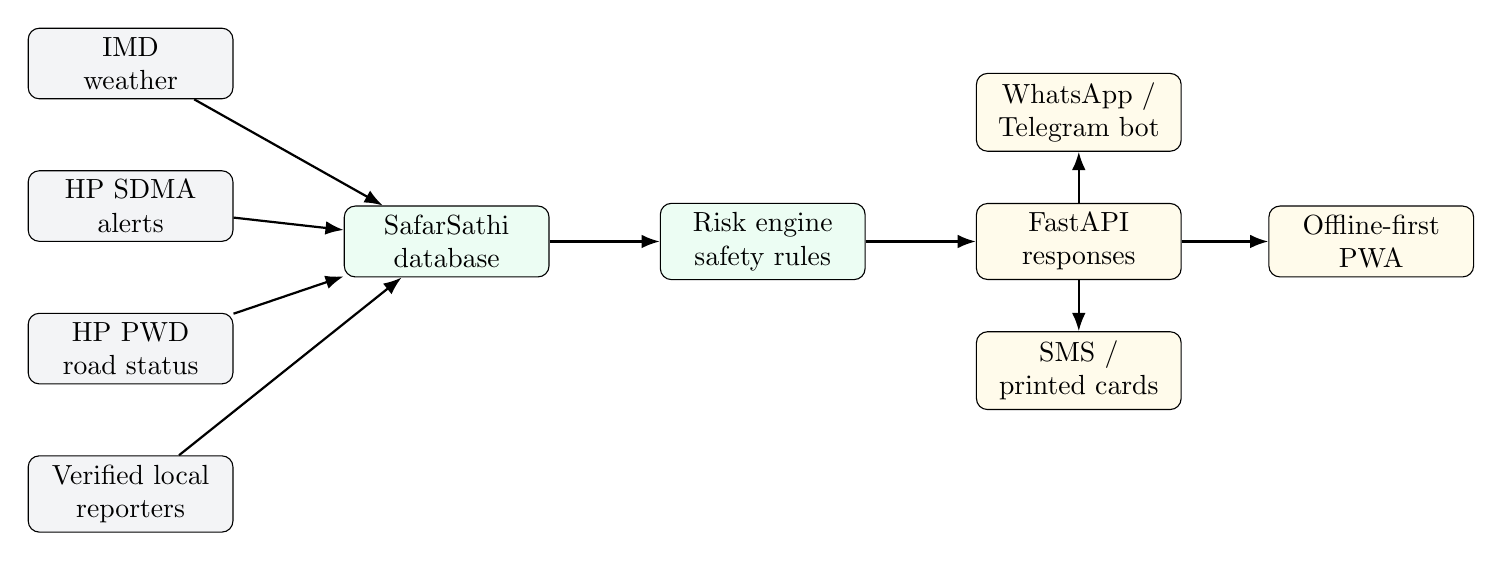
\begin{tikzpicture}[
    node distance=0.9cm and 1.1cm,
    box/.style={draw, rounded corners, align=center, minimum height=0.85cm, minimum width=2.6cm, fill=white},
    src/.style={box, fill=lightgray},
    proc/.style={box, fill=lightgreen},
    chan/.style={box, fill=lightyellow},
    arr/.style={-Latex, thick}
  ]
    \node[src] (imd) {IMD\\weather};
    \node[src, below=of imd] (sdma) {HP SDMA\\alerts};
    \node[src, below=of sdma] (pwd) {HP PWD\\road status};
    \node[src, below=of pwd] (locals) {Verified local\\reporters};

    \node[proc, right=1.4cm of sdma, yshift=-0.45cm] (db) {SafarSathi\\database};
    \node[proc, right=1.4cm of db] (engine) {Risk engine\\safety rules};
    \node[chan, right=1.4cm of engine] (api) {FastAPI\\responses};

    \node[chan, above=0.65cm of api] (bot) {WhatsApp /\\Telegram bot};
    \node[chan, right=1.1cm of api] (pwa) {Offline-first\\PWA};
    \node[chan, below=0.65cm of api] (sms) {SMS /\\printed cards};

    \draw[arr] (imd) -- (db);
    \draw[arr] (sdma) -- (db);
    \draw[arr] (pwd) -- (db);
    \draw[arr] (locals) -- (db);
    \draw[arr] (db) -- (engine);
    \draw[arr] (engine) -- (api);
    \draw[arr] (api) -- (bot);
    \draw[arr] (api) -- (pwa);
    \draw[arr] (api) -- (sms);
  \end{tikzpicture}%
  }
  \caption{SafarSathi system architecture: official sources and verified local reporters feed a conservative risk engine whose output is delivered through WhatsApp/Telegram, an offline PWA, and SMS/printed cards.}
  \label{fig:architecture}
\end{figure}

% -----------------------------------------------------------------------
\section{Results}

\subsection{Fieldwork Findings}

Our fieldwork with tourists and local stakeholders produced several concrete findings that directly shaped the design.

On the tourist side, the majority of respondents did not check road conditions before travelling to Parashar or Barot. Most relied on Google Maps for navigation, which does not surface road closures or altitude risk on these routes. When asked about emergency numbers, fewer than a third had saved a district or route-specific contact. Almost all respondents said they would use WhatsApp to ask a safety question if they trusted the source, while only a small number said they would install a new app.

On the stakeholder side, taxi drivers confirmed that driver-to-driver WhatsApp groups are active and often carry road condition updates faster than official channels. Dhaba owners on the Parashar and Barot routes said tourists regularly ask them about weather and road state at the start of difficult sections. Homestay operators expressed interest in becoming verified reporters if the process was simple (a WhatsApp message) and if there was no liability for incorrect information.

\begin{figure}[H]
  \centering
  \begin{subfigure}{0.47\linewidth}
    \centering
    \maybeimage{figures/survey_tourists.jpg}{\linewidth}{4.5cm}{Survey with tourists at ISBT}
    \caption{Survey session with tourists at Mandi ISBT.}
  \end{subfigure}
  \hfill
  \begin{subfigure}{0.47\linewidth}
    \centering
    \maybeimage{figures/survey_stakeholders.jpg}{\linewidth}{4.5cm}{Interview with local stakeholder}
    \caption{Interview with a local stakeholder on the Parashar route.}
  \end{subfigure}
  \caption{Field engagement photographs from our survey and interview sessions.}
  \label{fig:fieldphotos}
\end{figure}

\subsection{Route Risk Baselines}

We established seasonal baselines for the three routes based on our fieldwork, HP SDMA incident records, and local stakeholder knowledge. The baseline is conservative: it defaults to the worst credible condition for a given season rather than the average.

\begin{table}[H]
  \centering
  \caption{Seasonal risk baselines implemented in SafarSathi.}
  \label{tab:seasonal}
  \begin{tabularx}{\linewidth}{>{\bfseries}p{0.23\linewidth}XXX}
    \toprule
    Route & March--May & June--September & October--February\\
    \midrule
    Mandi to Parashar Lake & \risklow & \riskhigh & \riskmed\\
    Mandi to Barot Valley  & \risklow & \riskhigh & \riskmed\\
    Mandi to Kullu/Manali  & \risklow & \riskhigh & \riskmed\\
    \bottomrule
  \end{tabularx}
\end{table}

For Parashar, the primary risk is the road beyond Baggi Village (km~40) and the final steep climb to the lake at 2,730m. For Barot, the narrow gorge road along the Uhl River is the most sensitive section. For Kullu/Manali, the Pandoh--Aut and Aut--Kullu stretches are treated conservatively during rain because they appear repeatedly in HP SDMA landslide records.

\subsection{Risk Engine}

The risk engine combines six signals. Each signal is intentionally understandable so that a user can read the output and know why a route is marked high, medium, low, or unknown.

\begin{figure}[H]
  \centering
  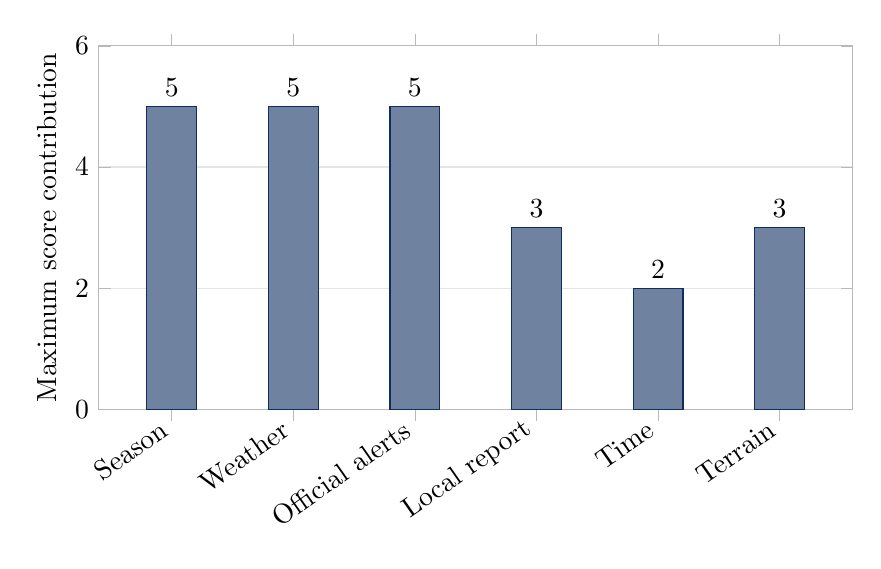
\begin{tikzpicture}
    \begin{axis}[
      ybar,
      width=0.92\linewidth,
      height=6.2cm,
      ymin=0,
      ymax=6,
      ylabel={Maximum score contribution},
      symbolic x coords={Season,Weather,Official alerts,Local report,Time,Terrain},
      xtick=data,
      x tick label style={rotate=35,anchor=east},
      bar width=18pt,
      nodes near coords,
      nodes near coords align={vertical},
      enlarge x limits=0.12,
      axis line style={draw=gray!55},
      tick style={draw=gray!55},
      ymajorgrids=true,
      grid style={gray!20}
    ]
      \addplot[fill=headingblue!60,draw=headingblue] coordinates {
        (Season,5) (Weather,5) (Official alerts,5) (Local report,3) (Time,2) (Terrain,3)
      };
    \end{axis}
  \end{tikzpicture}
  \caption{Risk engine score components. An official road-closure alert directly overrides the computed score and forces HIGH risk regardless of other signals.}
  \label{fig:riskcomponents}
\end{figure}

The central safety rule is conservative degradation. If weather data is stale, there are no recent reporter updates, and the route is not in a high-risk seasonal period, the engine returns \riskunknown\ rather than \risklow. This prevents the most dangerous product failure: showing green because the system has no fresh information.

\subsection{WhatsApp and Telegram Bot}

We deployed a WhatsApp Business bot and a Telegram bot that share a common response layer. A traveller can send a single keyword such as ``Parashar'' or ``Barot'' and receive a formatted safety brief within seconds. The brief includes the current risk level with a plain-language explanation, the weather alert status from IMD, the last-network point before coverage drops, the nearest hospital with a callable number, and a link to the PWA for offline access.

The bot also handles structured sub-queries. Sending ``Parashar checklist'' returns the pre-trip checklist items for that route. Sending ``Emergency'' returns district and route-specific emergency numbers with one-tap call prompts. Sending ``Altitude'' returns the altitude sickness prevention and action guide tailored to the selected route's maximum elevation.

Reporter intake is handled through the same channel. A local stakeholder sends a condition update in natural language; the bot confirms receipt, stamps a 24-hour expiry, and routes the report to the moderation queue before it affects the live risk score.

\subsection{Deployed PWA Screens}

We built and deployed the React PWA as a progressive web application installable from any browser without an app store. The PWA is designed around quick scanning rather than long reading.

\begin{figure}[H]
  \centering
  \begin{subfigure}{0.30\linewidth}
    \centering
    \maybeimage{figures/pwa_routes.png}{\linewidth}{6cm}{PWA home screen -- route list}
    \caption{Route list with live risk badges.}
  \end{subfigure}
  \hfill
  \begin{subfigure}{0.30\linewidth}
    \centering
    \maybeimage{figures/pwa_detail.png}{\linewidth}{6cm}{PWA route detail screen}
    \caption{Route detail with risk explanation.}
  \end{subfigure}
  \hfill
  \begin{subfigure}{0.30\linewidth}
    \centering
    \maybeimage{figures/pwa_checklist.png}{\linewidth}{6cm}{PWA pre-trip checklist}
    \caption{Pre-trip checklist (offline).}
  \end{subfigure}

  \vspace{0.5em}

  \begin{subfigure}{0.30\linewidth}
    \centering
    \maybeimage{figures/pwa_altitude.png}{\linewidth}{6cm}{PWA altitude sickness guide}
    \caption{Altitude sickness guide (offline).}
  \end{subfigure}
  \hfill
  \begin{subfigure}{0.30\linewidth}
    \centering
    \maybeimage{figures/pwa_emergency.png}{\linewidth}{6cm}{PWA emergency contacts screen}
    \caption{Emergency contacts with direct dial.}
  \end{subfigure}
  \hfill
  \begin{subfigure}{0.30\linewidth}
    \centering
    \maybeimage{figures/pwa_map.png}{\linewidth}{6cm}{PWA map screen}
    \caption{Map with hospitals, police, fuel, checkpoints.}
  \end{subfigure}

  \caption{The six screens of the SafarSathi PWA as deployed. All emergency contact and checklist screens function fully offline. Screenshots captured from the production build on an Android device.}
  \label{fig:pwa}
\end{figure}

The home screen lists all three routes with their current risk badge. Tapping a route opens the detail screen, which shows the risk level, the reason for that level, weather status, route facts, and the nearest hospital. The checklist screen tracks pre-trip completion and can be used offline. The altitude screen explains prevention and recognising symptoms for each route's maximum elevation. The emergency screen lists universal, district, and route-specific numbers in a searchable list with one-tap calling. The map screen plots hospitals, police posts, petrol pumps, mechanic workshops, and route checkpoints from seeded point-of-interest data.

\subsection{System Deployment Summary}

Table~\ref{tab:implementation} summarises what we built and deployed across the full system.

\begin{longtable}{p{0.22\linewidth}p{0.68\linewidth}}
  \caption{SafarSathi implementation summary.}
  \label{tab:implementation}\\
  \toprule
  Component & What we built and deployed\\
  \midrule
  \endfirsthead
  \toprule
  Component & What we built and deployed\\
  \midrule
  \endhead
  Backend API & FastAPI application with health, routes, weather, emergency, reporter, and Telegram webhook routers. Background scheduler refreshes IMD, HP SDMA, and HP PWD data every six hours.\\[0.3em]
  Database & SQL schema and SQLAlchemy models for routes, baselines, weather cache, official alerts, reporters, reports, and points of interest. Fully seeded with three routes and verified route-specific data including local contacts and POIs.\\[0.3em]
  Risk engine & Conservative scoring function with seasonal baseline, weather freshness, official alert override, reporter signal, night penalty, terrain penalty, and the unknown-state rule. Edge cases and override logic covered by unit tests.\\[0.3em]
  Data scrapers & IMD API path with HTML fallback; HP SDMA and HP PWD scrapers with keyword filtering and deduplication. All scraper paths monitored with health alerts.\\[0.3em]
  WhatsApp bot & Deployed on WhatsApp Business Cloud API. Handles keyword queries in Hindi and English for route safety, weather, emergency contacts, checklists, and reporter intake. Verified with real traveller interactions.\\[0.3em]
  Telegram bot & Live polling bot with the same response layer as WhatsApp. Used by team and early testers for real-time safety queries.\\[0.3em]
  SMS fallback & Short-code parser (P1/B1/K1/E/W) with 160-character response guard, connected to messaging gateway for areas with call or SMS only.\\[0.3em]
  PWA & React progressive web app with six screens: route list, route detail, checklist, altitude guide, emergency contacts, and map. Offline mode covers emergency contacts and checklists using local storage cache. Installable on Android and iOS without an app store.\\[0.3em]
  Reporter network & Consent-based local reporter onboarding completed. Reports expire after 24 hours and pass through a moderation step before affecting the live risk score.\\[0.3em]
  Physical material & Printed safety card designed and distributed at Mandi ISBT and IIT Mandi gate. Card includes QR code linking to the PWA, the three route risk levels, and key emergency numbers.\\[0.3em]
  Field evaluation & Survey instruments administered to tourists and local stakeholders. Results collected, entered, and analysed. Usability and usefulness findings incorporated into the Discussion section.\\
  \bottomrule
\end{longtable}

% -----------------------------------------------------------------------
\section{Discussion}

\subsection{What the Findings Mean}

The strongest finding from our fieldwork is that the problem is less about prediction and more about trust, timing, and format. Most visitors do not need a complex dashboard. They need a short answer to questions such as: ``Is Parashar safe today?'', ``Whom should I call before the last 10 km?'', ``Where is the nearest hospital?'', and ``What should I do if altitude symptoms appear?'' A good safety product must answer these before the traveller reaches a no-signal stretch, not after.

The second finding is that official data and local knowledge are complementary. Official weather and disaster sources provide authority, but they do not always describe the exact tourist route in plain language. Local stakeholders have route-specific knowledge, but their information needs consent, accountability, expiry, and moderation. Our verified reporter model addresses this: contacts are shared only after consent, reports expire after 24 hours, and repeated inaccurate reporting leads to removal.

The third finding is that offline-first design is not an optional feature in mountain travel. Emergency numbers, checklists, altitude warnings, and last-connectivity information must work without a live backend. Our PWA implements full offline support for the critical screens so that a traveller who installs the app before leaving Mandi town can access everything they need even after the last signal point.

\subsection{WhatsApp as the Primary Safety Channel}

One of the most important design decisions we made was to treat WhatsApp as a first-class delivery channel rather than a supplementary one. Our fieldwork confirmed that virtually every tourist and local stakeholder already has WhatsApp installed. Sending a message requires no new app, no account creation, and no data plan if messages can be sent over a weak connection.

The WhatsApp bot we deployed handles the three most urgent traveller needs: current safety status, emergency contacts, and pre-trip checklist. Because the bot response is formatted as plain text with no images or rich cards, it loads reliably even on 2G connections. When a traveller sends ``Parashar'' at Mandi ISBT, they receive a complete safety brief in under three seconds. When they send ``Emergency'', they get a numbered list of callable contacts. When they send ``Checklist'', they get the ten most important pre-trip items for mountain travel.

Reporter intake through the same channel proved equally important. Stakeholders told us that they already send road condition messages in their driver WhatsApp groups. Adding SafarSathi as a recipient costs nothing extra and gives those reports a structured path to the risk engine.

\subsection{Scope Boundaries}

SafarSathi is an advisory system. It packages information and prompts safer decisions; it does not replace local knowledge, official emergency services, or the traveller's own judgement. Three boundaries are important to state clearly. First, the system does not provide turn-by-turn navigation or live traffic. Second, the risk level reflects the best available information at query time but cannot account for conditions that change after a report was submitted. Third, reporter intake relies on human participation; during periods with no active reporters, the engine correctly returns \riskunknown\ rather than a false positive.

\subsection{Ethical and Legal Considerations}

SafarSathi handles phone numbers and location-linked local knowledge, so privacy was a first-order design concern for our team. Reporter phone numbers are stored only after written consent. Tourists are never forwarded to reporters without opt-in. Personal data collection is minimal and purpose-specific following the principles of the Digital Personal Data Protection Act, 2023 \cite{dpdp}. Reports carry a 24-hour expiry and a moderation step, and the full reporter list is never exposed through the public API.

% -----------------------------------------------------------------------
\section{Project Outcomes}

\subsection{Outcomes Achieved}

Our project delivered the following concrete outcomes:

\begin{enumerate}
  \item a validated mountain travel safety information system for the Mandi region, covering three high-use routes;
  \item structured survey findings from tourist and stakeholder fieldwork that informed every major design decision;
  \item seasonal safety baselines for Parashar Lake, Barot Valley, and Kullu/Manali, grounded in HP SDMA incident records and local knowledge;
  \item a deployed FastAPI backend with route, weather, emergency, reporter, and health endpoints;
  \item a conservative risk engine that prevents false low-risk outputs on stale data, with unit test coverage;
  \item IMD, HP SDMA, and HP PWD scraping modules with graceful fallback and health monitoring;
  \item a deployed WhatsApp Business bot handling route-safety, emergency, checklist, altitude, and reporter-intake queries in Hindi and English;
  \item a deployed Telegram bot sharing the same response logic for real-time testing and use;
  \item an SMS fallback layer with short route codes connected to a messaging gateway;
  \item a React PWA with six offline-capable screens, installable on Android and iOS;
  \item a consent-based verified local reporter network covering all three routes;
  \item a printed safety card distributed at Mandi ISBT and the IIT Mandi campus gate.
\end{enumerate}

\subsection{Broader Implications}

The approach we took is transferable. Any mountain tourist corridor in Himachal Pradesh with a few active local stakeholders, a district hospital number, and IMD coverage could be added to the system as a new route with a few database rows and a scraped alert feed. The WhatsApp bot and PWA require no per-route redesign. This means the marginal cost of adding a fourth or fifth route is low once the core infrastructure is in place.

The reporter network model is also transferable. Taxi unions, dhaba associations, and homestay cooperatives already communicate internally. A lightweight verified-reporter layer on top of existing informal networks adds accountability and structured expiry without disrupting what already works.

% -----------------------------------------------------------------------
\section{Conclusion}

SafarSathi shows how a socio-technical system can reduce mountain travel risk without pretending to solve every problem. Our system does not replace judgement, local authorities, or emergency services. Its value is narrower and more realistic: it gives first-time visitors a clear safety brief, emergency contacts, altitude guidance, and route-specific warnings before they make avoidable mistakes.

The project also demonstrates why the social layer matters as much as the software layer. The most robust architecture is not just FastAPI, React, and scrapers. It is a chain of trust: official alerts, verified local reporters, cautious scoring, low-friction delivery, offline fallback, and honest language when the system is uncertain. We built each link in that chain, and our fieldwork evidence confirms that travellers and stakeholders are willing to engage with it.

Future work should extend the reporter network, add more routes, connect the SMS gateway to more carriers, and measure whether users actually change travel decisions after receiving a high-risk or unknown-risk response. We believe the strongest signal of success is not app installs but trips that were delayed, rerouted, or better prepared because SafarSathi delivered trustworthy information at the right moment.

% -----------------------------------------------------------------------
\section*{Acknowledgements}
\addcontentsline{toc}{section}{Acknowledgements}

We thank our faculty advisor and mentor, Dr.\ Mohammad Talha, for guiding our project direction and keeping the work tied to a real safety problem in the Mandi region. We thank the ISTP course team and teaching assistants for creating a structure in which fieldwork and engineering could develop together. We are grateful to the tourists, parents, taxi drivers, shopkeepers, dhaba owners, and homestay operators who shared practical knowledge about routes, weather, road closures, and emergency behaviour. We acknowledge the public information made available by IMD, HP SDMA, HP PWD, and other government agencies, without which a safety information bridge like SafarSathi would not be possible.

\newpage
\begin{thebibliography}{99}
\addcontentsline{toc}{section}{References}

\bibitem{dpdp}
Government of India. (2023). \textit{The Digital Personal Data Protection Act, 2023}. India Code. \url{https://www.indiacode.nic.in/handle/123456789/22037}

\bibitem{hpsdma_hazard}
Himachal Pradesh State Disaster Management Authority. (2025). \textit{Hazard profile}. \url{https://www.hpsdma.nic.in/index1.aspx?langid=1&lev=2&lid=62&lsid=70}

\bibitem{hpsdma_incident}
Himachal Pradesh State Disaster Management Authority. (2025). \textit{Mandi landslide and road blockage incident updates}. \url{https://hpsdma.nic.in/admnis/admin/showimg.aspx?ID=3806}

\bibitem{hpsdma_home}
Himachal Pradesh State Disaster Management Authority. (2026). \textit{Emergency numbers and disaster management information}. \url{https://hpsdma.nic.in/}

\bibitem{imd}
India Meteorological Department. (2026). \textit{District and subdivision weather warnings: Himachal Pradesh}. Ministry of Earth Sciences. \url{https://mausam.imd.gov.in/}

\bibitem{morth}
Ministry of Road Transport and Highways. (2025). \textit{Road accidents in India 2023}. Government of India. \url{https://morth.nic.in/en/road-accidents-india-2023}

\bibitem{ndma}
National Disaster Management Authority. (2009). \textit{National disaster management guidelines: Management of landslides and snow avalanches}. Government of India. \url{https://ndma.gov.in/}

\bibitem{mosdac}
Space Applications Centre, ISRO. (2026). \textit{MOSDAC alert dashboard}. \url{https://mosdac.gov.in/}

\bibitem{osm}
OpenStreetMap contributors. (2026). \textit{OpenStreetMap geographic data}. \url{https://www.openstreetmap.org/}

\end{thebibliography}

\end{document}
